\documentclass[11pt]{article}
\usepackage[utf8]{inputenc}
\usepackage[spanish,es-tabla]{babel}
\usepackage{amsmath,cancel}
\usepackage{amsfonts}
\usepackage{amssymb}
\usepackage{listings}
\usepackage{xcolor}
\usepackage{tabularx}
\usepackage{adjustbox}
\spanishdecimal{.}
\usepackage{graphicx}
\usepackage{float}
\usepackage[lmargin=2.5cm,rmargin=2.5cm,top=2.5cm,
bottom=2cm]{geometry}
\newcommand{\nombre}{Oscar}
\newcommand{\fecha}{9 de mayo del 2026}
\newcommand{\tituloPractica}{}
%%%%%%%%%%%%%%%%%%%%%%%%%%%%%%%%%%%%%%%%%%%%%%
\begin{document}
\begin{titlepage}
\begin{center}
\vspace*{2\baselineskip}
\hrule height 3pt
\vspace*{0.5\baselineskip}
{\Large \textbf{UNIVERSIDAD DE GUADALAJARA}}\\[0.1cm]
{\large \textbf{CENTRO UNIVERSITARIO DE CIENCIAS EXACTAS E INGENIER\'IAS}}
\vspace*{0.5\baselineskip}
\hrule
\vspace*{3\baselineskip}
\includegraphics[width=0.2\textwidth]{udg}
\vspace*{2\baselineskip}\\
{\large\textbf{ Algor\'itmos Bio-Inspirados \\ Msc. Rob\'otica e Inteligencia Artificial}
\vspace*{\baselineskip}\\
{\large Algoritmo 8 --- ILS N-Dimensional \vspace{1cm} \\
\begin{tabular}{p{4cm}p{8cm}}
\hline \hline
Nombre del alumno:  & Oscar Alberto Gallo Garc\'ia \\
C\'odigo del alumno:  & 218357704 \\
Profesor: & Dr. Carlos Alberto Lopez Franco \\
 \hline \hline
\end{tabular}
\vfill
\fecha
\end{center}
\newpage
\end{titlepage}

\tableofcontents
\newpage

\section{Resumen}

Se implement\'o el algoritmo \textit{Iterated Local Search} (ILS) para optimizaci\'on continua en $n$ dimensiones. El m\'etodo alterna ciclos de b\'usqueda local estoc\'astica (escalada de colinas aleatoria) y perturbaci\'on para escapar de m\'inimos locales. Se evaluaron cuatro casos sobre funciones altamente multimodales con m\'as de tres \'optimos locales: minimizaci\'on y maximizaci\'on de la funci\'on de Rastrigin en 2 dimensiones con gr\'aficas de superficie y contorno, y minimizaci\'on y maximizaci\'on de Rastrigin y Ackley en 4 dimensiones.

\section{Metodolog\'ia}

El algoritmo ILS fue propuesto como meta-heur\'istica general para escapar de \'optimos locales. La idea central es que una b\'usqueda local de alta calidad, combinada con perturbaciones que modifiquen la soluci\'on de forma significativa, puede explorar el espacio de soluciones de manera m\'as eficiente que reinicios aleatorios completos.

\subsection{B\'usqueda local estoc\'astica}

Se utiliza escalada de colinas con pasos aleatorios (\textit{stochastic hill climbing}). En cada iteraci\'on interna se genera una soluci\'on vecina $\mathbf{x}'$ perturbando la soluci\'on actual con un desplazamiento uniforme de magnitud m\'axima $p$ en cada dimensi\'on:

\[
x'_d = \text{clamp}\!\left(x_d + u_d,\; \ell_{\min},\; \ell_{\max}\right), \qquad u_d \sim \mathcal{U}(-p, p)
\]

El movimiento se acepta \'unicamente si mejora el valor de la funci\'on objetivo:

\[
\mathbf{x} \leftarrow
\begin{cases}
\mathbf{x}' & \text{si } f(\mathbf{x}') \prec f(\mathbf{x}) \\
\mathbf{x}  & \text{en caso contrario}
\end{cases}
\]

donde $\prec$ denota $<$ en minimizaci\'on y $>$ en maximizaci\'on.

\subsection{Perturbaci\'on}

Para escapar del \'optimo local encontrado, se aplica una perturbaci\'on aleatoria de mayor magnitud $F \gg p$:

\[
x'_d = \text{clamp}\!\left(x_d + v_d,\; \ell_{\min},\; \ell_{\max}\right), \qquad v_d \sim \mathcal{U}(-F, F)
\]

La perturbaci\'on mueve la soluci\'on a una cuenca de atracci\'on diferente del espacio de b\'usqueda.

\subsection{Criterio de aceptaci\'on}

Se emplea un criterio voraz: la nueva soluci\'on (tras la b\'usqueda local desde el punto perturbado) se acepta como nueva mejor soluci\'on s\'olo si estrictamente mejora a la incumbente:

\[
\mathbf{x}^* \leftarrow \mathbf{x}_{\text{new}} \quad \text{si } f(\mathbf{x}_{\text{new}}) \prec f(\mathbf{x}^*)
\]

\subsection{Algoritmo ILS}

\begin{enumerate}
    \item Inicializar: $\mathbf{x}_0 \sim \mathcal{U}(\ell_{\min}, \ell_{\max})^n$.
    \item Aplicar b\'usqueda local: $\mathbf{x}^* \leftarrow \textsc{BL}(\mathbf{x}_0)$.
    \item Repetir hasta $t_{\max}$ iteraciones:
    \begin{enumerate}
        \item Perturbar: $\mathbf{x}' \leftarrow \textsc{Perturb}(\mathbf{x}^*, F)$.
        \item Aplicar b\'usqueda local: $\mathbf{x}_{\text{new}} \leftarrow \textsc{BL}(\mathbf{x}')$.
        \item Si $f(\mathbf{x}_{\text{new}}) \prec f(\mathbf{x}^*)$: actualizar $\mathbf{x}^* \leftarrow \mathbf{x}_{\text{new}}$.
    \end{enumerate}
    \item Retornar $\mathbf{x}^*$.
\end{enumerate}

\subsection{Par\'ametros}

\begin{table}[H]
\centering
\begin{tabular}{lcc}
\hline\hline
Par\'ametro & 2D & 4D \\
\hline
$p$ (paso de b\'usqueda local) & 0.1 & 0.1 \\
$F$ (fuerza de perturbaci\'on) & 2.0 & 2.0 \\
$n_{\text{local}}$ (iters.\ de b\'usqueda local) & 500 & 1000 \\
$t_{\max}$ (iteraciones ILS)   & 50  & 100  \\
\hline\hline
\end{tabular}
\caption{Par\'ametros utilizados en todos los experimentos.}
\end{table}

\subsection{Funciones de prueba}

Ambas funciones son altamente multimodales con m\'as de tres \'optimos locales y un \'unico \'optimo global en el origen.

\begin{align}
f_{\text{rastrigin}}(\mathbf{x}) &= 10n + \sum_{j=1}^{n}\bigl[x_j^2 - 10\cos(2\pi x_j)\bigr] \notag\\[4pt]
f_{\text{ackley}}(\mathbf{x}) &= -20\exp\!\left(-0.2\sqrt{\tfrac{1}{n}\sum x_j^2}\right) - \exp\!\left(\tfrac{1}{n}\sum\cos(2\pi x_j)\right) + 20 + e \notag
\end{align}

\section{Resultados}

\subsection{Minimizaci\'on 2D}

\subsubsection{Funci\'on de Rastrigin}

M\'inimo global en $\mathbf{x}^* = (0,0)$ con $f(\mathbf{x}^*) = 0$. La topolog\'ia de valles peri\'odicos genera cientos de m\'inimos locales separados por barreras. El ILS logra escapar de los \'optimos locales cercanos y converge pr\'acticamente al \'optimo global: mejor soluci\'on $(-2.93\times10^{-3},\,5.5\times10^{-4})$, $f = 1.76\times10^{-3}$.

\begin{figure}[H]
\centering
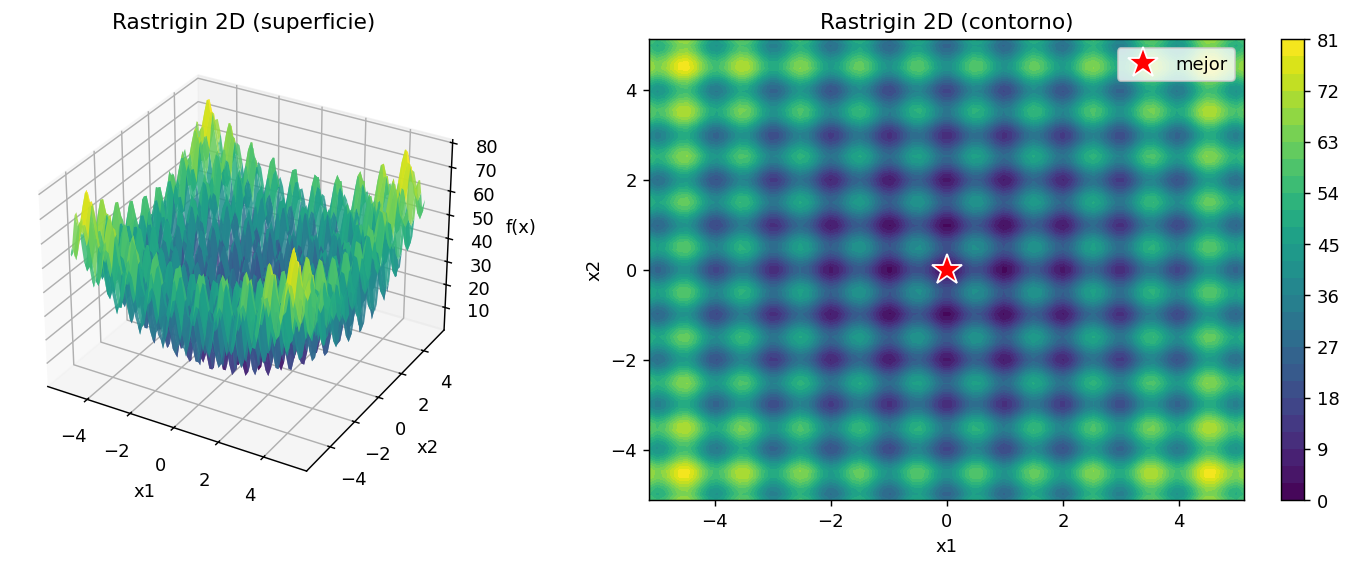
\includegraphics[width=14cm]{figs/ILS_min_rastrigin.png}
\caption{Minimizaci\'on de la funci\'on de Rastrigin. La cuadr\'icula de m\'inimos locales peri\'odicos constituye el principal reto; la estrella roja indica la mejor soluci\'on hallada por el ILS.}
\end{figure}

\subsection{Maximizaci\'on 2D}

\subsubsection{Rastrigin Negativa}

Se maximiza $-f_{\text{rastrigin}}(\mathbf{x})$, cuyo m\'aximo global es en $(0,0)$ con valor $0$. El ILS localiza el m\'aximo con alta precisi\'on: mejor soluci\'on $(-1.4\times10^{-3},\,-1.36\times10^{-3})$, $f = -7.56\times10^{-4}$.

\begin{figure}[H]
\centering
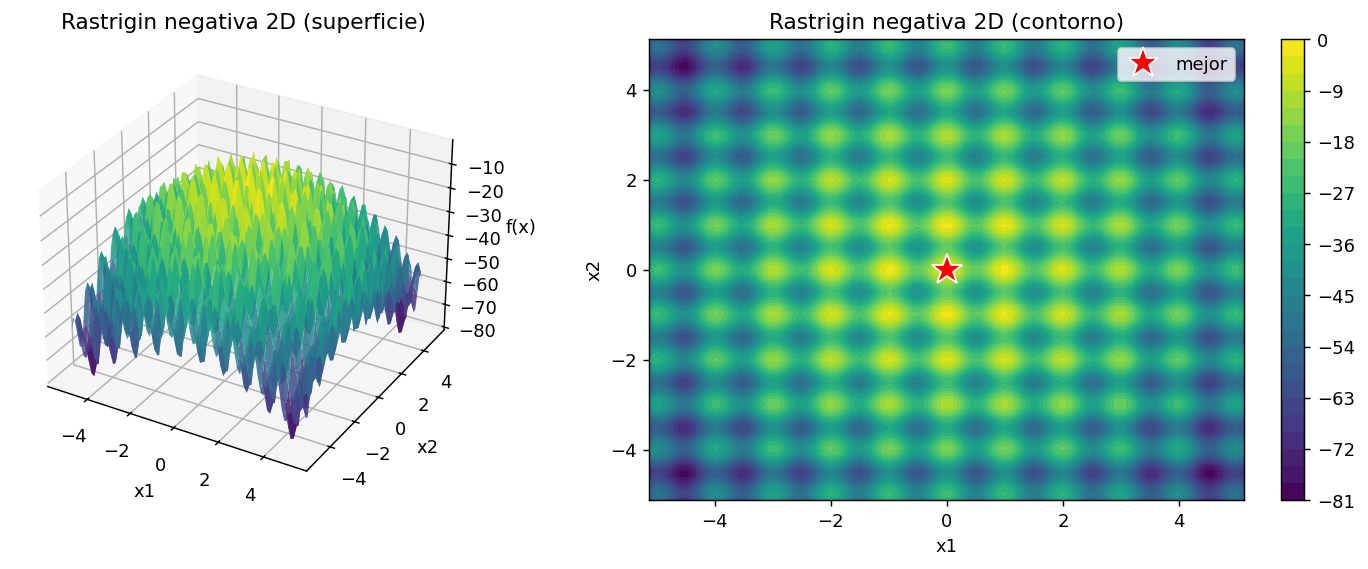
\includegraphics[width=14cm]{figs/ILS_max_rastrigin.png}
\caption{Maximizaci\'on de la Rastrigin negativa. La cuadr\'icula de m\'aximos locales id\'enticos rodea el m\'aximo global en el origen; el ILS lo localiza con error del orden de $10^{-3}$.}
\end{figure}

\subsection{Minimizaci\'on N-Dimensional (4D)}

\begin{table}[H]
\centering
\begin{tabular}{lp{8.5cm}r}
\hline\hline
Funci\'on & Mejor soluci\'on & $f(\hat{\mathbf{x}})$ \\
\hline
Rastrigin & $[0.98902,\;0.01281,\;0.02011,\;0.01438]$ & $1.156$ \\[3pt]
Ackley    & $[-3.82{\times}10^{-3},\;1.98{\times}10^{-3},\;-9.94{\times}10^{-3},\;-0.92593]$ & $1.842$ \\
\hline\hline
\end{tabular}
\caption{Resultados de minimizaci\'on en 4 dimensiones. Rastrigin queda en un m\'inimo local de periodo 1; Ackley queda cerca del \'optimo global aunque no lo alcanza debido a la asimetr\'ia introducida por el punto de inicio.}
\end{table}

\subsection{Maximizaci\'on N-Dimensional (4D)}

Se maximizan las versiones negadas de las funciones anteriores.

\begin{table}[H]
\centering
\begin{tabular}{lp{8.5cm}r}
\hline\hline
Funci\'on & Mejor soluci\'on & $f(\hat{\mathbf{x}})$ \\
\hline
$-$Rastrigin & $[1.00027,\;3.5{\times}10^{-4},\;6.11{\times}10^{-3},\;-1.48{\times}10^{-3}]$ & $-1.008$ \\[3pt]
$-$Ackley    & $[-1.202{\times}10^{-2},\;3.24{\times}10^{-3},\;8.41{\times}10^{-3},\;5.06{\times}10^{-3}]$ & $-0.035$ \\
\hline\hline
\end{tabular}
\caption{Resultados de maximizaci\'on en 4 dimensiones. $-$Ackley converge muy cerca del \'optimo global ($f \approx 0$); $-$Rastrigin queda atrapado en un m\'aximo local de periodo 1.}
\end{table}

\section{Conclusi\'on}

El ILS demostr\'o ser capaz de escapar de \'optimos locales en funciones altamente multimodales: en 2D tanto Rastrigin (minimizaci\'on) como Rastrigin negativa (maximizaci\'on) convergieron al vecindario inmediato del \'optimo global con errores del orden de $10^{-3}$, lo cual representa una mejora significativa frente a una b\'usqueda local sin perturbaci\'on que quedar\'ia atrapada en el primer \'optimo local visitado.\\\\
En 4 dimensiones, el rendimiento fue asim\'etrico entre funciones. Ackley en maximizaci\'on alcanz\'o $f \approx -0.035$, muy cercano al \'optimo global en $(0,0,0,0)$, gracias a la estructura suave de su paisaje de b\'usqueda en las cercan\'ias del origen. Rastrigin en 4D present\'o mayor dificultad: la cuadr\'icula de \'optimos locales peri\'odicos de periodo 1 genera barreras que el esquema de perturbaci\'on uniforme no siempre logra superar, resultando en soluciones con $f \approx 1$ en lugar de $0$.\\\\
La efectividad del ILS depende cr\'iticamente de la relaci\'on entre la fuerza de perturbaci\'on $F$ y la escala de los \'optimos locales. Con $F = 2.0$ y periodo $1$ de Rastrigin, es probable que la perturbaci\'on lleve la soluci\'on a un \'optimo local adyacente en lugar de a una cuenca lejana. Reducir $F$ para la b\'usqueda local e incrementarlo s\'olo en la perturbaci\'on, o emplear un esquema de perturbaci\'on adaptativo que aumente $F$ cuando no hay mejora, podr\'ia mejorar la exploraci\'on en funciones con m\'ultiples escalas.

\end{document}
